\documentclass[12pt, a4paper]{article}
\usepackage{amssymb, amsmath, amsthm} % matematikfunktionalitet
\usepackage[danish]{babel}
\usepackage{lipsum}
\usepackage[margin=2.5cm]{geometry}
\usepackage{parskip}
\usepackage{graphicx} %Titlepage
\usepackage[colorlinks = true,linkcolor = blue,urlcolor  = blue,citecolor = blue,anchorcolor = blue]{hyperref} %Titlepage - ændrer formateringen af links
\usepackage{tikz}
\usepackage{pgfgantt}
\usetikzlibrary{shapes, arrows}
\usepackage{pdflscape}
\usepackage{float}


\title{Projektbeskrivelse}
\author{Jeppe, Alexander, Andreas, David}
\date{}

\begin{document}
\maketitle
\section{Problemanalyse - intro}
    \begin{itemize}
    \item Samfundsmæssigt
    \item Brandsikkerhed
    \item Fraværsregistrering 
    \item modernisering af IT Systemer og forbedret infrastruktur.
    \end{itemize}
\section{Problemidentifikation}
\subsection{idegenerering}
\subsubsection{Mindmap}
Vi har anvendt et mindmap til at danne et overblik over, hvilke problemer vi i dette projekt kan bearbejde.
\begin{figure}[H]
    \centering
    \resizebox{\columnwidth}{!}{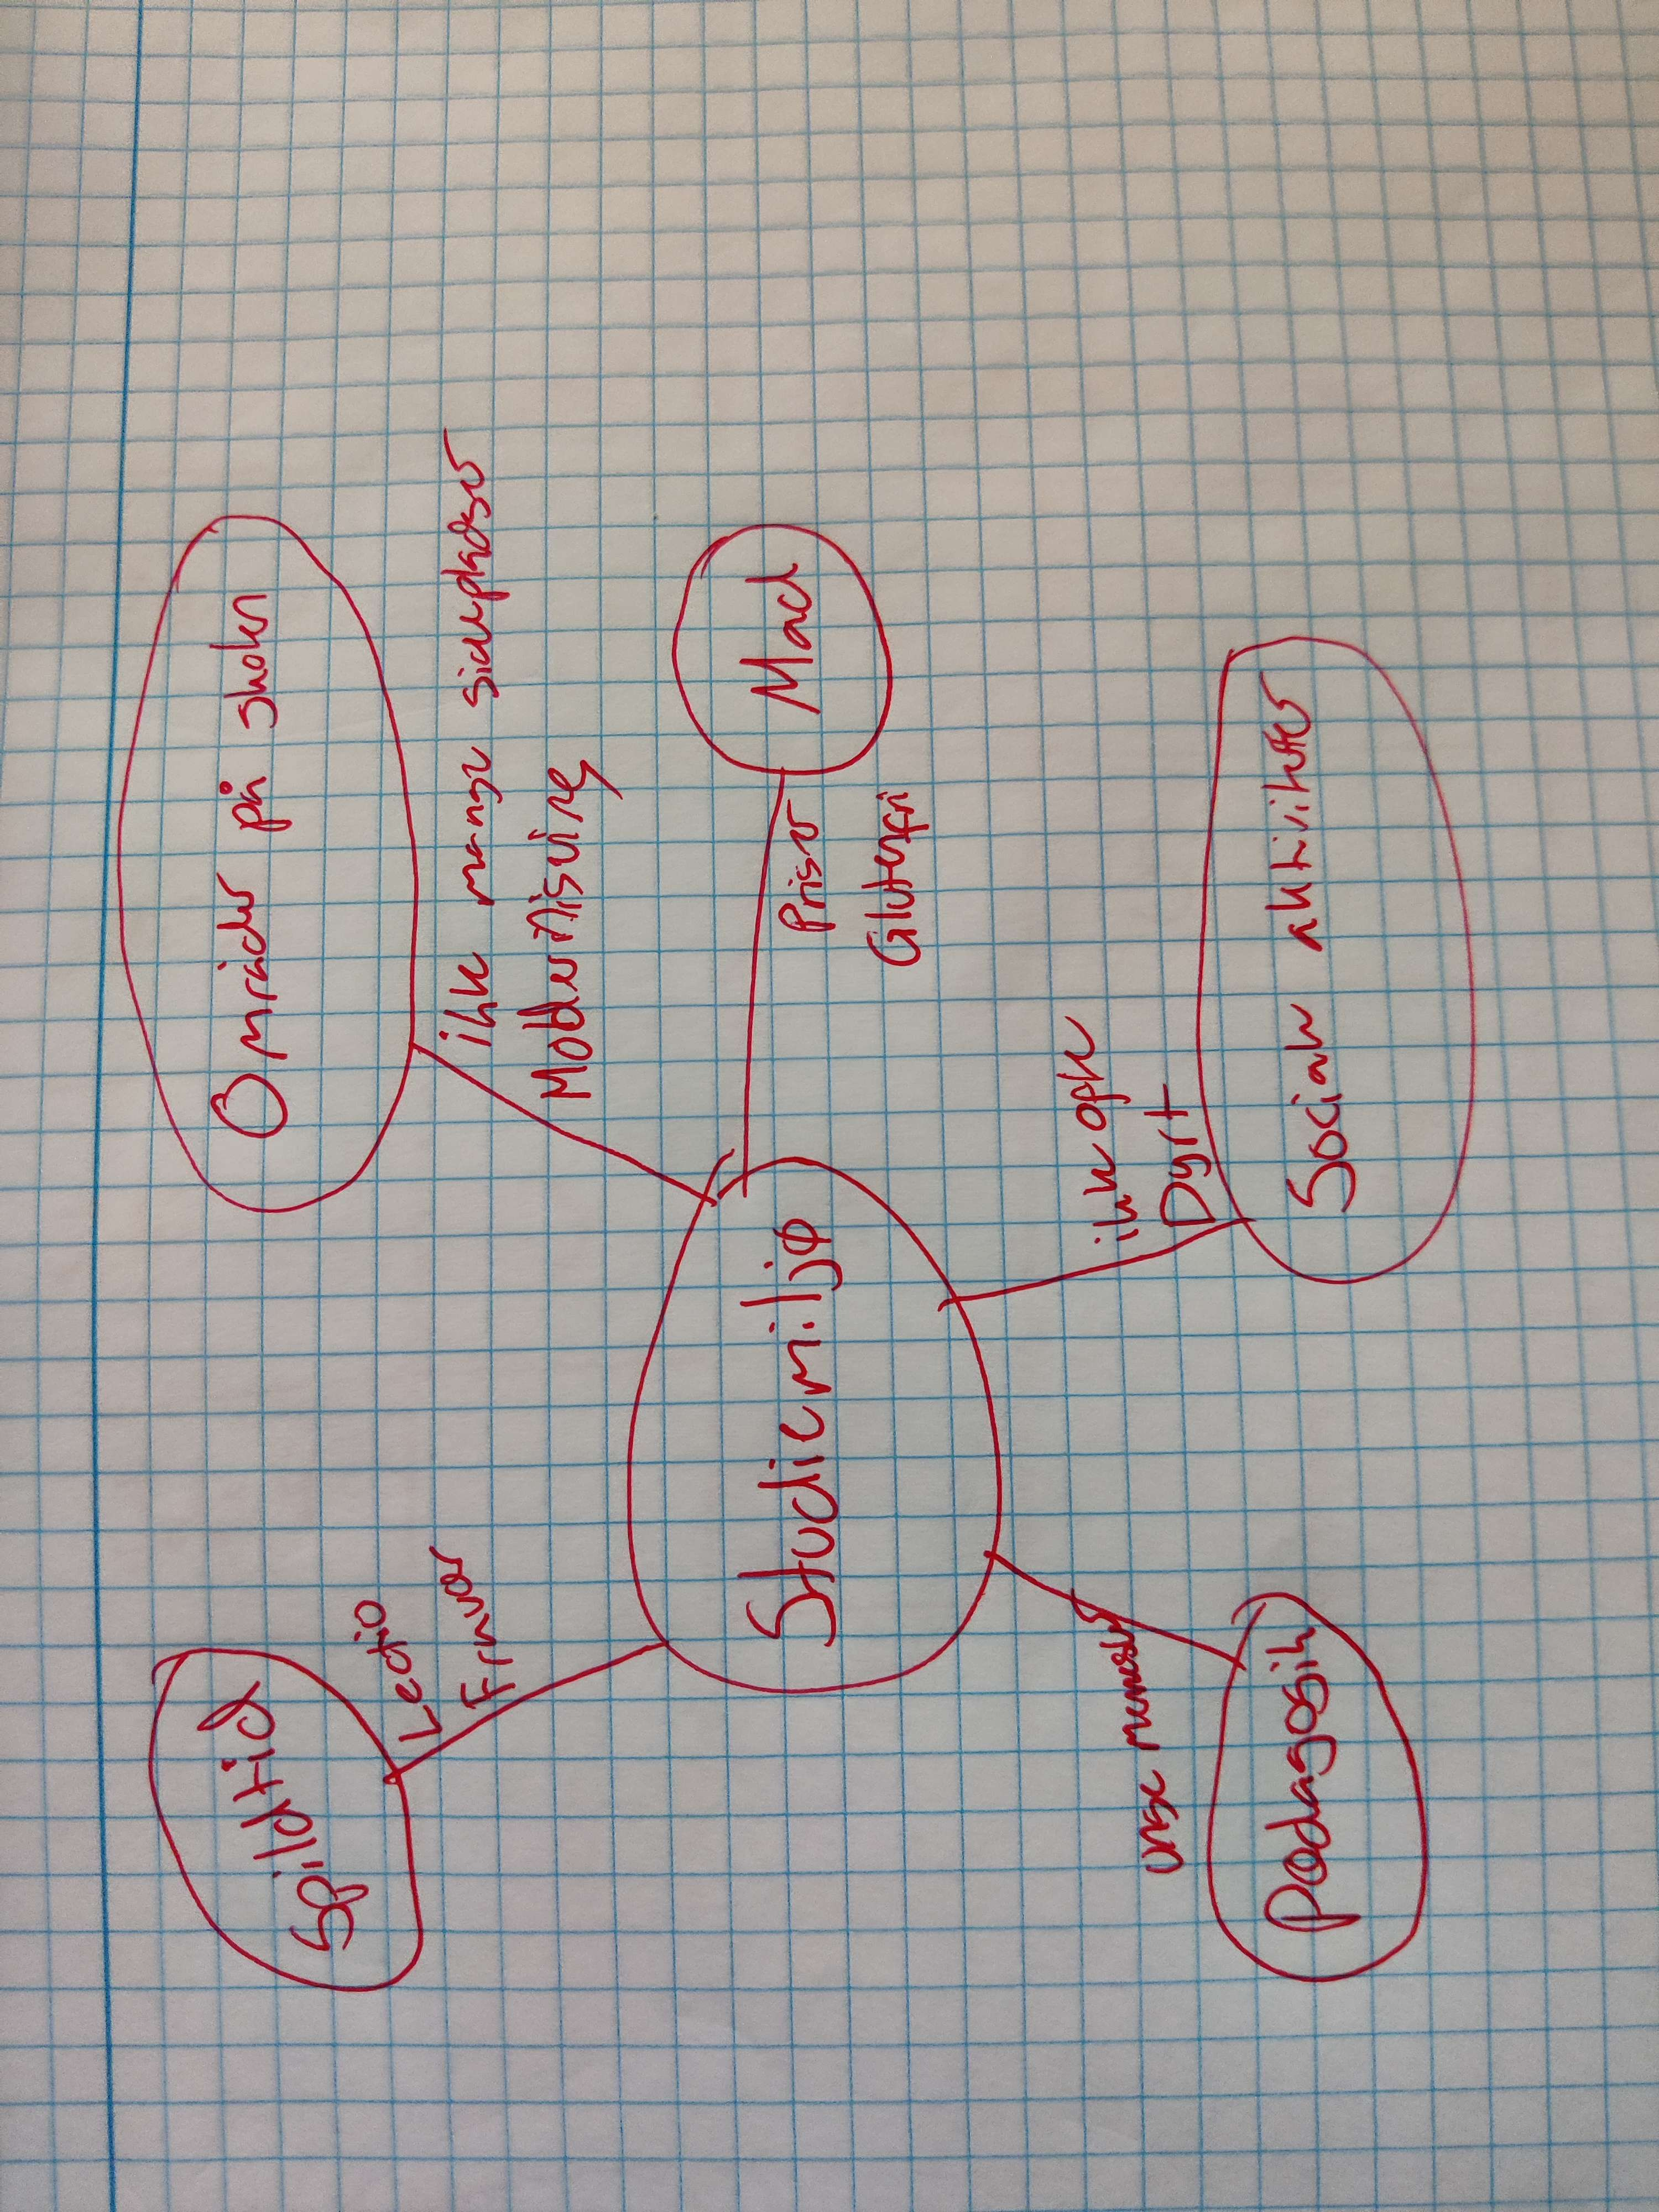
\includegraphics[angle =-90]{assets/mindmap.jpg}}
    \caption{Viser det anvende mindmap.}
\end{figure}

\subsubsection{Lyskurven}
    Efter vi lavede Mindmappet, valgte vi at benytte os af lyskurve-modellen til at sorterer i vores ideer. Lyskurven er et godt værktøj, som man bruger til at sortere i ens problemstillinger.
    Lyskurven fungerer ved, at man opstiller tre kategorier for at inddele ens ideer efter, hvor (tænkt) brugbare ideerne er. Så, man tildeler de problemer, man i gruppen gerne vil arbejde videre med og ser potientiale i, i den grønne kategori.
    Så har man også en gul kategori, som man bruger til ideer, man ikke er helt sikker på kan lykkeds, men de er i en backup-fase, så de kan tages i brug, hvis ens grønne ideer går i vasken.
    Til sidst har man den røde kategori, her befinder de ideer, man i gruppen har valgt at kasserer. Vores Lyskurve så således ud: 

\begin{table}[H]
    \centering
    \begin{tabular}{ll}
    \hline
    Spildtid,  områder på skole& Grøn \\
    \hline
    Pædagogik & Gul \\
    \hline
    Sociale aktiviteter, mad & Red
    \end{tabular}
    \caption{Viser et meget abstrakt lyskurvediagram i form af en tabel; det vi anvendte \label{fig:lyskurven}}
    \end{table}
\subsection{Identificering af nøgleproblem}
I vores lyskurvediagram (se tabellen \ref{fig:lyskurven}) har vi to i den grønne, gode, kategori, ergo skal vi endvidere vælge en af disse at arbejde med. 
Vi har anvendt følgende spørgsmål til at indsnævre valget:
\begin{enumerate}
    \item Hvorfor er det her interessant?
    \item Hvem er det interessant for?
    \item Er det noget, vi laver for vores egen fornøjelses skyld?
    \item Er det noget, som en bestemt gruppe i samfundet kan have gavn af, eller er det noget, der er til gavn for alle?\\*** Spørgsmålene er hentet fra "projektarbejdet"-bogen via Systime \footnote{\url{https://projektarbejdet.systime.dk/?id=145}}
\end{enumerate}
Således har vi besvaret spørgsmålene:
\begin{itemize}
\item 1) Tidspild er interessant, fordi det særligt vedrører 1.x-klassen, da det er en meget stor klasse med tilsvarende få lærer, ergo er der på forhånd en dårlig tidsallokering per elev per modul samt er der mange ting, der gøres på ineffektive muligheder; ergo er casen oplagt. Områder på skolen er også interessant, da det berører os alle, men det er ikke en videre spændende problemstilling at fordybe i.
\item 2) Redundans - jf. besvarelsen ovenover
\item 3) Ja, bl.a. da vi er kede af, hvor meget tid vi spilder. De fysiske områder kunne godt trænge til lidt modernisering.
\item 4) Produktet med er til gavn for samtlige af det danske kongeriges studerende og deres respektive undervisere. Forbedring af de fysiske områder ville først og fremmest komme os til gode.
\end{itemize}

Ergo vælger vi at arbejde videre med tidspildsproblematikken, da denne er mest interessant baseret på svarene.
\section{Produktudkast}
    Vores Lectio Renovering modernisser HTX' IT-systemer. Det vil vi blandt andet gøre ved at lancere et identitesbaseret system på RFID, hvilket gør en ende på spildt tid med fraværstagning og eventuelt falsk fravær, da dette automatisk registreres, når du scanner dit ID-kort. 
\subsection{Lokale-Booking-System}
    Vores Lokale-Booking-System vil revolutionere måden, hvorpå vi booker lokaler. 
    Det vil gøre en ende på unødigt tidsspild, altså den tid, det tager at gå op på kontoret, frem og tilbage med nøgler.
\subsection{Smartdøre}
    Vores Smartdøre vil forbedre brandsikkerheden og fungerer sammen med booking-systemet og elevernes identifikationskort.
    I tilfælde af brand vil alle skolens døre låse op og lukke automatisk så alle rum bliver isoleret, og brænden bliver forsøgt kvalt. 
\subsection{Lectio Renovering}
    Det vil også sige, at hvis et lokale nu er låst, og uheldet er ude, hvor man skal flygte ud af et vindue, der er bag et aflåst lokale, vil man nu kunne spare potientelt tabte liv.

    \begin{landscape}
\section{Tidsplan}
\begin{figure}[H]
    \centering
    \begin{ganttchart}[vgrid,hgrid,time slot format=little-endian,expand chart=\columnwidth]{1.3.2024}{14.5.2024}
        \gantttitlecalendar{year, month=name, week=9, day} \ganttnewline
        \ganttgroup{Forberedelse}{1.3.2024}{7.3.2024} \\
        \ganttgroup{Produktudvikling}{7.3.2024}{14.5.2024} \\
        \ganttgroup{Rapportudformning}{7.3.2024}{14.5.2024} \\
        % \ganttlink{elem3}{elem4}
    \end{ganttchart}
    \caption{Viser Gantt-Diagram over vores foreløbige tidsplan. Se appendiks med projektbeskrielse.}
\end{figure}
\end{landscape}
\end{document}

